%%%%%%%%%%%%%%%%%%%%%%%%%%%%%%%%%%%%%%%%%%%%%%%%%%%%%%%%%%%%%%%%%%%%%%%%%%%%%%%%%%%%%%%%%%%%%%
% Template Beamer Sugestivo para Projetos no Senac
% by ezefranca.com
% Based on MIT Beamer Template
% As cores laranja e azul seguem o padrao proposto no manual de uso da identidade visual senac
%%%%%%%%%%%%%%%%%%%%%%%%%%%%%%%%%%%%%%%%%%%%%%%%%%%%%%%%%%%%%%%%%%%%%%%%%%%%%%%%%%%%%%%%%%%%%% 

%\documentclass{beamer} %voce pode usar este modelo tambem
\documentclass[handout,t]{beamer}
\usepackage{graphicx,url}
\usepackage[english]{babel}   
\usepackage[utf8]{inputenc}
\usepackage{wrapfig}
\usepackage[demo]{graphicx}
\usepackage{subcaption}
%\usepackage{colortbl}
\newtheorem{defn}{Definition}
\batchmode
% \usepackage{pgfpages}
% \pgfpagesuselayout{4 on 1}[letterpaper,landscape,border shrink=5mm]
\usepackage{amsmath,amssymb,enumerate,epsfig,bbm,calc,color,ifthen,capt-of}
\usetheme{Berlin}
\usecolortheme{senac}

\usepackage{lipsum}

\newcommand\blfootnote[1]{%
  \begingroup
  \renewcommand\thefootnote{}\footnote{#1}%
  \addtocounter{footnote}{-1}%
  \endgroup
}


\setbeamerfont{footnote}{size=\tiny}

%-------------------------Titulo/Autores/Orientador------------------------------------------------
\title[SCNet]{SCNet: \\Automatic Multi-Channel Genome Network \\Inference from Single-Cell RNA Sequences}
\author[Topics in Computational Biology (2019 Autumn)]{Shiyin Wang (wangshiy16@mails.tsinghua.edu.cn)}
\date{December 23, 2019}

%-------------------------Logo na parte de baixo do slide------------------------------------------
\pgfdeclareimage[height=0.7cm]{senac-logo}{uiuc.png}
\logo{\pgfuseimage{senac-logo}\hspace*{0.5cm}}

%-------------------------Este código faz o menuzinho bacana na parte superior do slide------------
\AtBeginSection[]
{
  \begin{frame}<beamer>
    \frametitle{Outline}
    \tableofcontents[currentsection]
  \end{frame}
}
\beamerdefaultoverlayspecification{<+->}
% -----------------------------------------------------------------------------
\begin{document}
% -----------------------------------------------------------------------------

%---Gerador de Sumário---------------------------------------------------------
\frame{\titlepage}
\section[]{}
\begin{frame}{Outline}
  \tableofcontents
\end{frame}
%---Fim do Sumário------------------------------------------------------------



% -----------------------------------------------------------------------------
\section{Introduction}
\subsection{Single-Cell RNA Sequencing}
\begin{frame}{What is single-cell RNA sequencing?}
\vspace{-0.4cm}
\begin{figure}
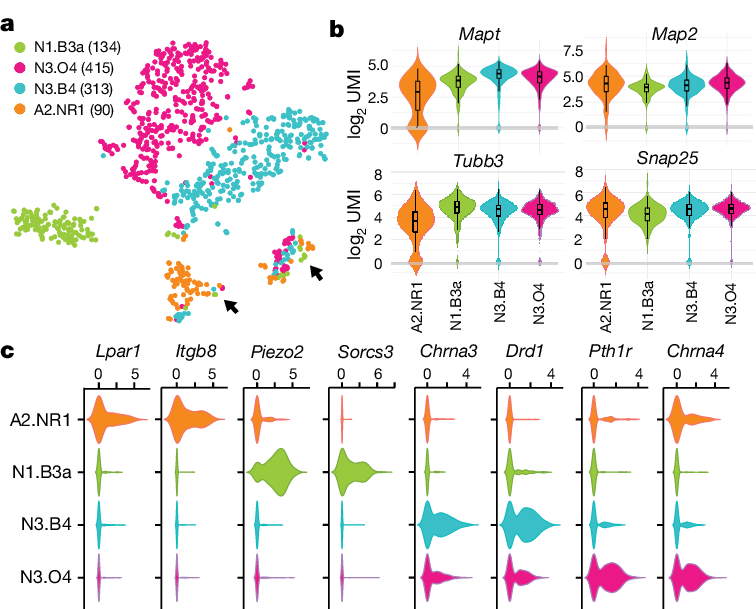
\includegraphics[width=0.65\columnwidth]{Single-cell-RNA-seq-of-four-iN-cell-populations-a-c-Cells-are-colour-coded-as.png}
\end{figure}
\vspace{-0.3cm}
\blfootnote{Tsunemoto, Rachel, et al. "Diverse reprogramming codes for neuronal identity." Nature 557.7705 (2018): 375.}
\end{frame}


\begin{frame}{Datasets}
\begin{figure}
  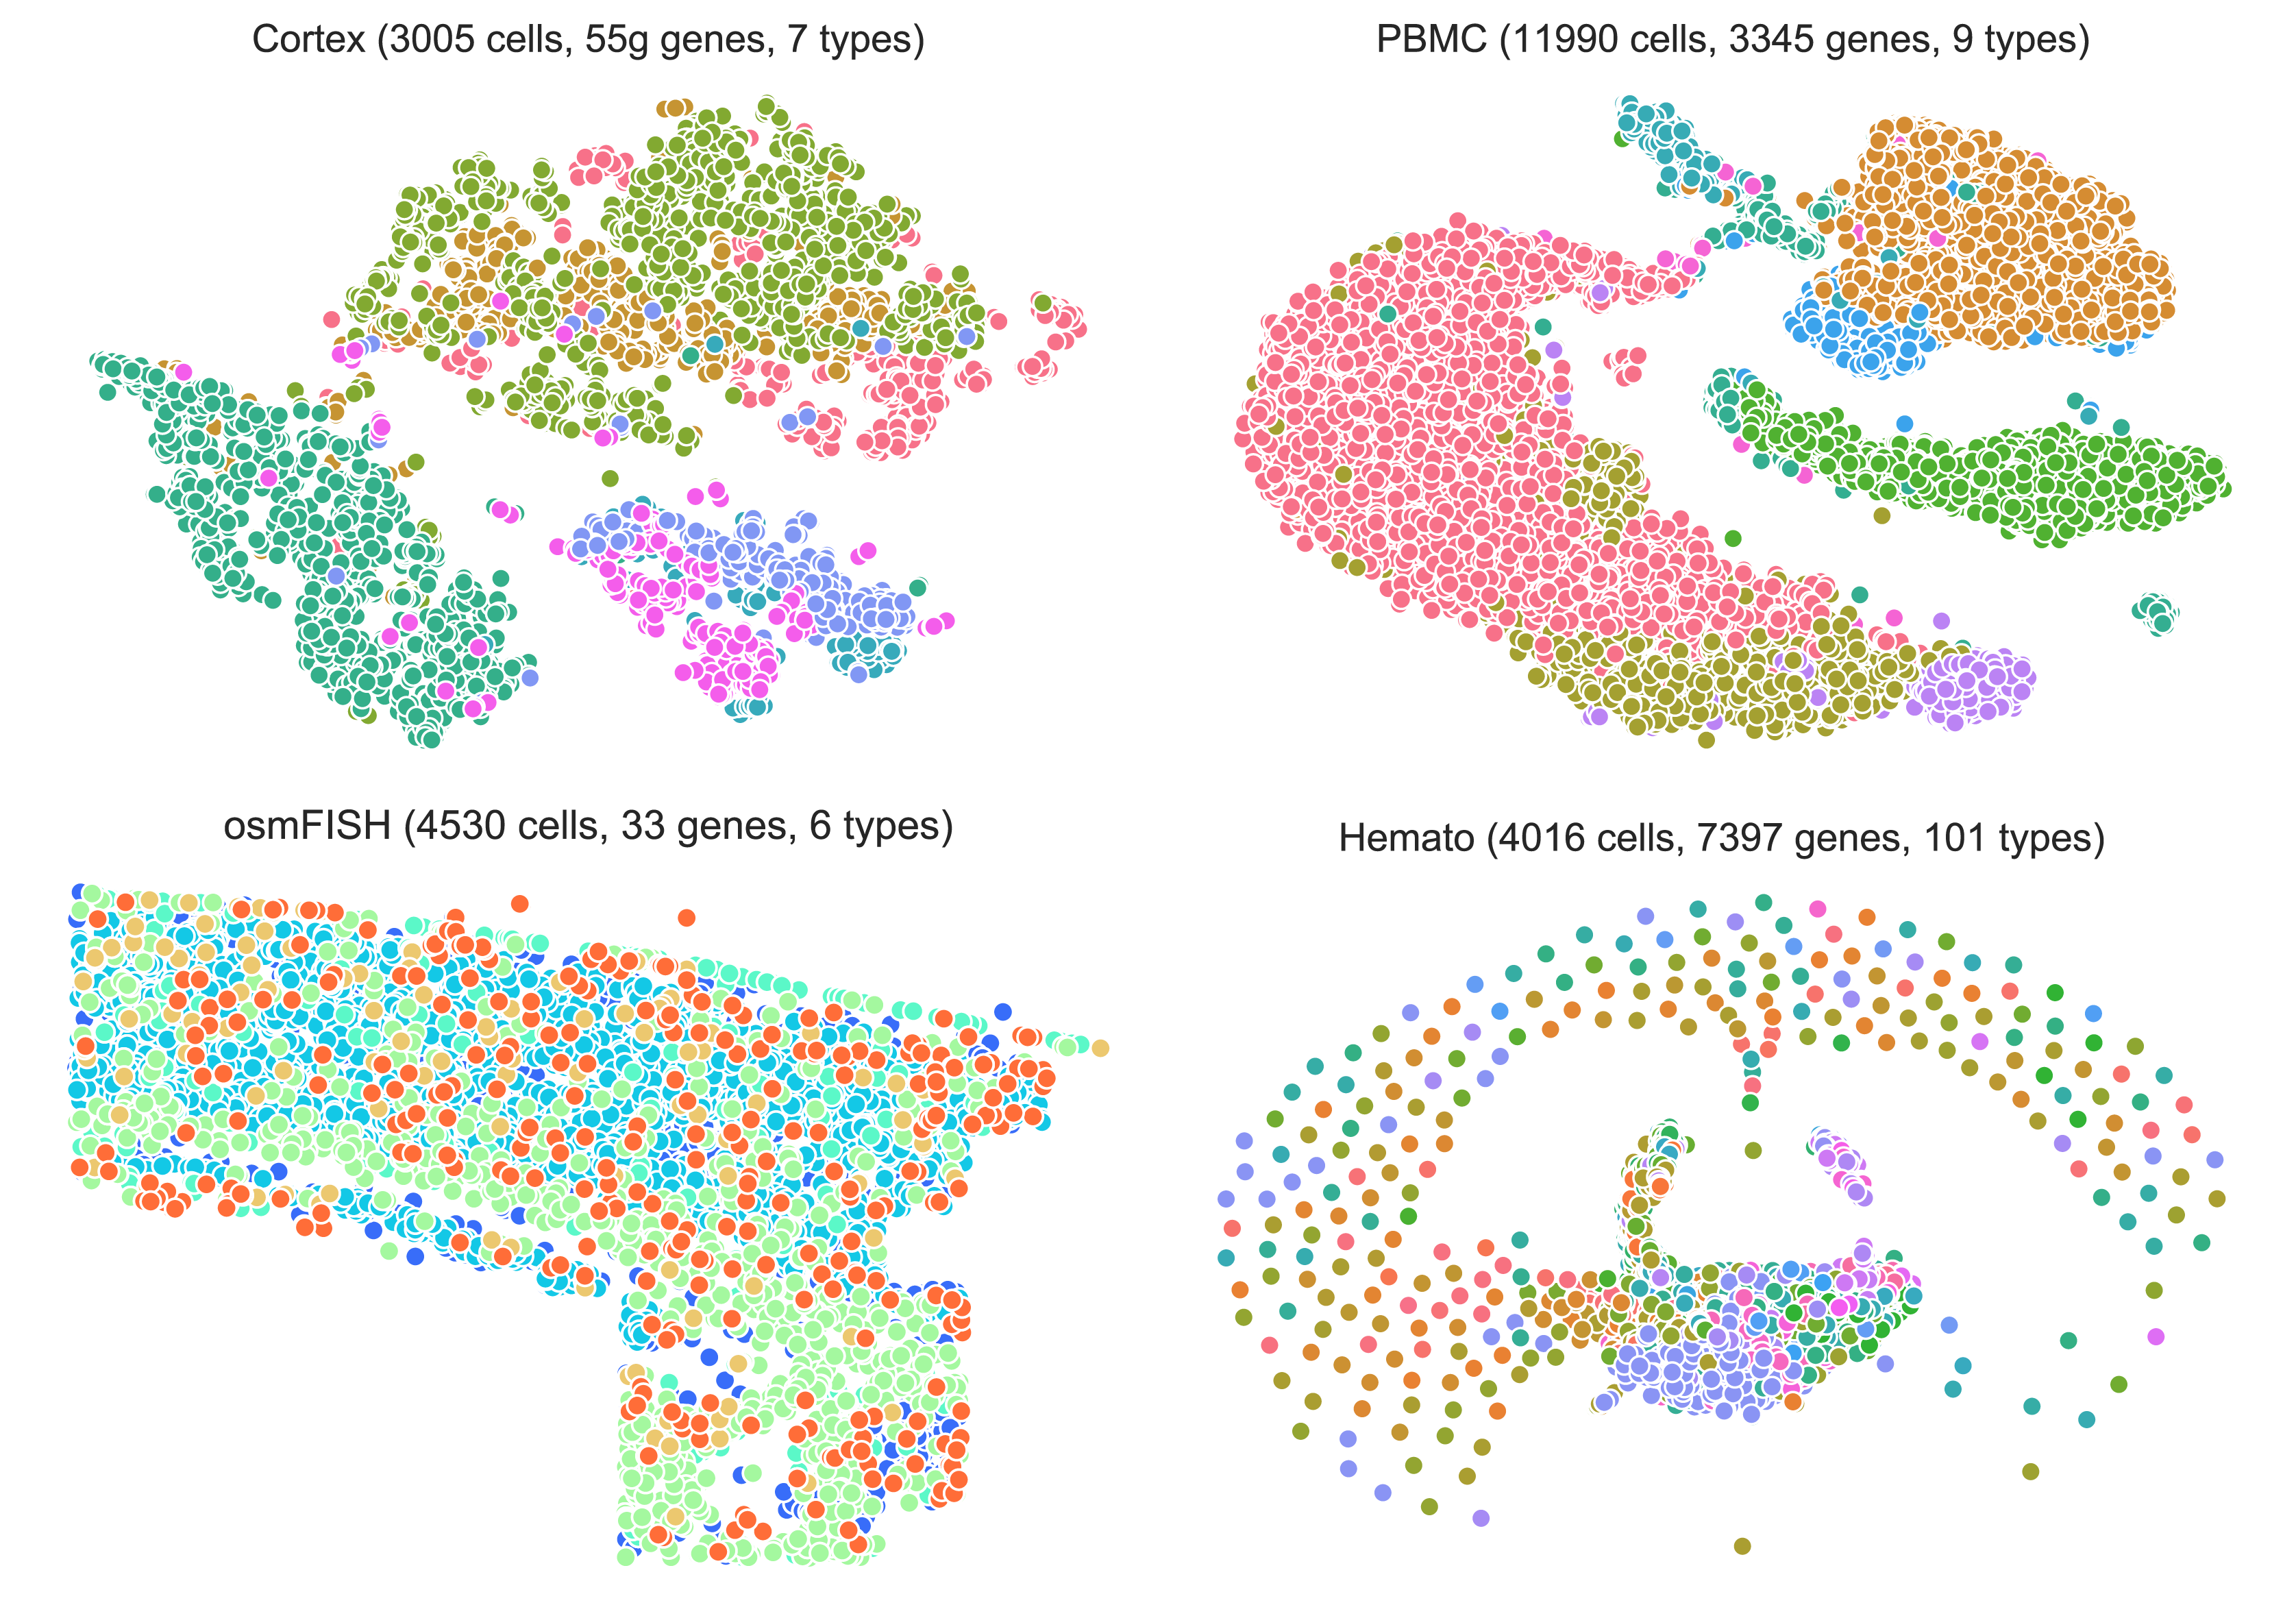
\includegraphics[width=0.8\columnwidth]{../figure/scatter.png}
\end{figure}
\end{frame}


\subsection{Mathematics Preliminaries}
\begin{frame}{Bayesian Methods}
\begin{figure}
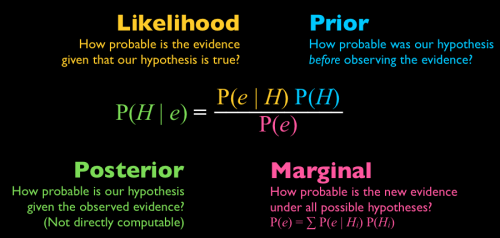
\includegraphics[width=\columnwidth]{bayes.png}
\end{figure}
\end{frame}

\begin{frame}{Markov Chain Monte Carlo}
\vspace{-0.3cm}
\begin{figure}
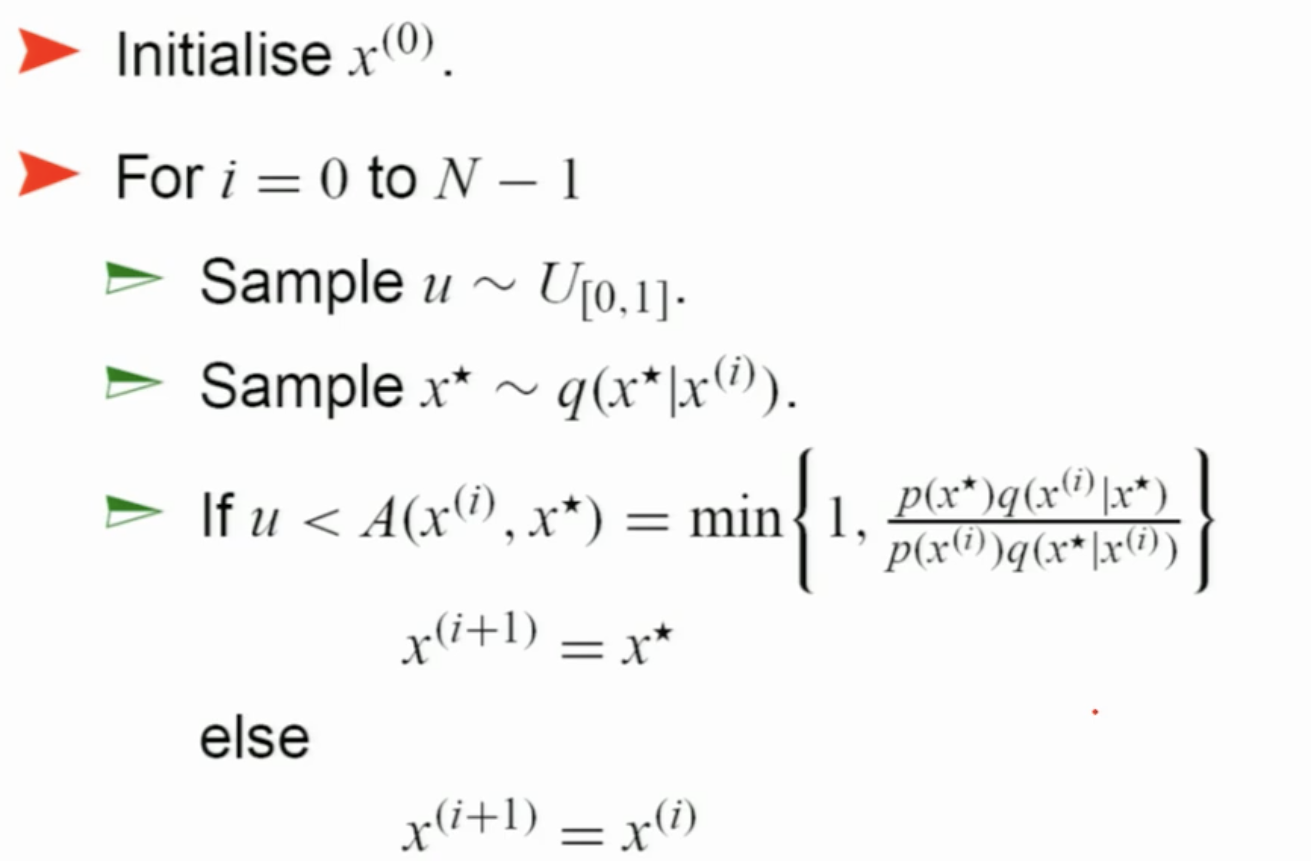
\includegraphics[width=0.7\columnwidth]{mcmc.png}
\end{figure}
\vspace{-0.1cm}
\blfootnote{Slide in CPSC 540, taught in 2013 at UBC by Nando de Freitas}
\end{frame}


%------------------------------------------------------------------------------

\section{Methods}

\subsection{Probabilistic models}

\begin{frame}{Choose Log-Scale to Model Gene Expression}
\vspace{-0.5cm}
\begin{figure}
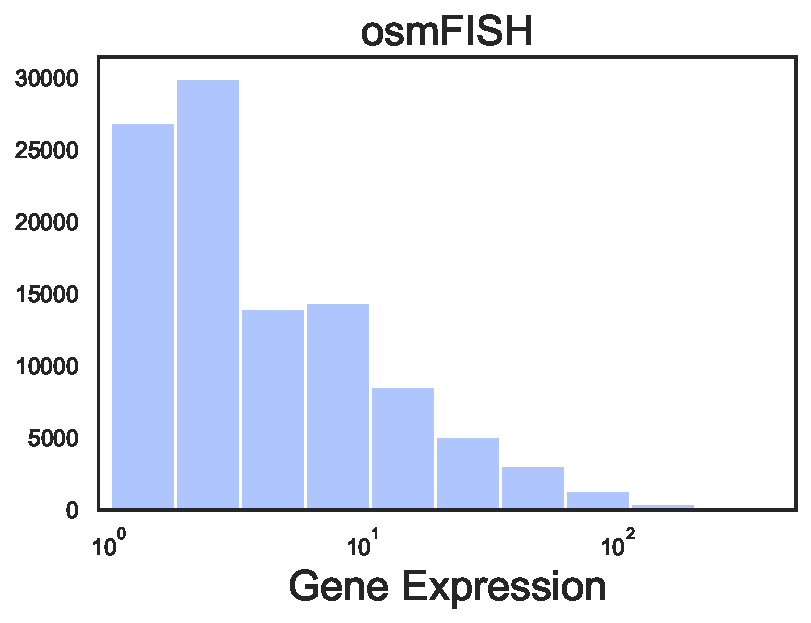
\includegraphics[width=0.7\columnwidth]{../figure/dist/osmFISH.pdf}
\end{figure}
\vspace{-0.1cm}
The support of X and Y is a non-negative, we use $log(X+1)$ instead of $log(X)$ to map it onto the log-scale non-negative space.
\end{frame}


\begin{frame}{Bayesian Hierarchical Linear Model}
X and Y are the expression profiles of two genes. The edge weights in the desired network correspond to the regression coefficient $k$ in the equation.
\begin{equation}
    \begin{array}{ll}
            log(Y+1) = k log(X+1) +\epsilon\\
            k \sim N(\beta, \sigma)\\
            \epsilon \sim N(0, \gamma^2)\\
    \end{array}
\end{equation}
This model estimates k from single-cell RNA sequencing records.
\end{frame}

\begin{frame}{Define Transition Probability through Edge Weights}
Once we have a weighted network, we can define the association probability between two nodes X and Y by a very trivial model.
\begin{equation}\begin{split}
   Pr(X& \rightarrow Y) = 1-\\
   &(1-w_{X, Y})\Pi_{a\in V}(1-w_{X, a}w_{a, Y})\Pi_{a\in V, b\in V}(1-w_{X, a}w_{a, b}w_{b, Y})
\end{split}\end{equation}
For simplicity, I expanded the search for three steps. Walk length is flexible to choose.
\end{frame}

\begin{frame}{Maximal Likelihood Optimization}
Bayesian hierarchical linear model and transition probability explain the network dynamics from two different angles. Now we can combine them together to infer the edge weights of networks $(V, E, W)$.
\begin{equation}
   maximize\ L(W; \Beta_k, \Sigma_k) = \sum_{v_1\in V} \sum_{v_2\in V} Pr_{N(\Beta_k, \Sigma_k)} (w=Pr(v_1\rightarrow v_2))
\end{equation}
Add regulation term $\lambda |V|$ to restrain the number of edges in the network.
\begin{equation}
   maximize\ L(W; \Beta_k, \Sigma_k) = \sum_{v_1\in V} \sum_{v_2\in V} Pr_{N(\Beta_k, \Sigma_k)} (w=Pr(v_1\rightarrow v_2)) - \lambda |V|
\end{equation}
\end{frame}


\subsection{Optimization}
\begin{frame}{Data Preprocessing - Normalization}
\begin{enumerate}
\item Retained the top genes ordered by variance as in [Lopez \textit{et al.}, 2018]\footnote{Lopez, R., Regier, J., Cole, M.B. et al. Deep generative modeling for single-cell transcriptomics. Nat Methods 15, 1053–1058 (2018) doi:10.1038/s41592-018-0229-2}
\item Normalize genes to standard Gaussian distribution $N(0, 1)$
\end{enumerate}
Reason for normalization to standard deviation: So that the regression coefficient in $Y=kX+\epsilon$ is $\hat{k} = \frac{cov(X, Y)}{var(X)} = cov(X, Y)$, which is exchangeable and bidirectional.
\end{frame}



%------------------------------------------------------------------------------


\section{Results}





%------------------------------------------------------------------------------

\section{Future Work}

\begin{frame}{Possible Directions}
\begin{itemize}
\item Theoretical analysis and case study to compare with other methods that derive networks from covariance matrix directly
\item Integrate existing knowledge from protein-protein interaction networks (STRING, OmniPATH, ConsensusPath, etc) as priors
\item Design better probability models
\item Make interactive transition videos
\end{itemize}
\end{frame}


\begin{frame}{Resources}
\begin{itemize}
\item 10x Genomics: Datasets providing single cell and spatial views of biological systems (\url{https://www.10xgenomics.com})
\end{itemize}
\end{frame}


%------------------------------------------------------------------------------

\section{Q \& A}
\begin{frame}{Questions \& Answers}
\vspace{-0.3cm}
\begin{figure}
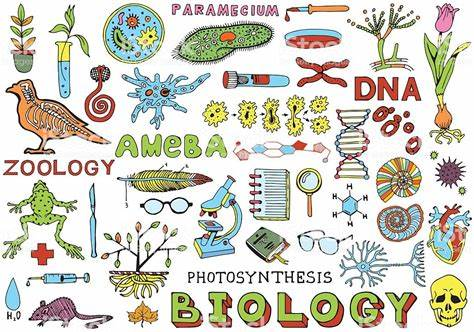
\includegraphics[width=0.85\columnwidth]{th.jpeg}
\end{figure}
\end{frame}

\end{document}
%------------------------------------------------------------------------------

